\documentclass[aps,pra,twocolumn,superscriptaddress,showpacs,floatfix]{revtex4-2}

\usepackage{amsmath,amssymb}
\usepackage{graphicx}
\usepackage{hyperref}
\usepackage{booktabs}
\usepackage{bm}
\usepackage{xcolor}
\usepackage{multirow}

\hypersetup{
  colorlinks=true,
  linkcolor=blue!60!black,
  citecolor=blue!60!black,
  urlcolor=blue!60!black,
  pdfauthor={Berkay Y{\"u}ksel Sayim},
  pdftitle={Sector-Dependent CHSH Violation in Fibonacci Anyons, and Finite-Size Topological–CHSH Mutual Information in 2D Lattice Models},
  pdfsubject={quant-ph; topological order; CHSH inequality; Fibonacci anyons},
  pdfkeywords={CHSH, topological order, Fibonacci anyons,
               mutual information, lattice gauge theory, finite-size scaling}
}

% Abkuerzungen
\newcommand{\braket}[1]{\langle #1 \rangle}
\newcommand{\ket}[1]{| #1 \rangle}
\newcommand{\bra}[1]{\langle #1 |}
\newcommand{\Ztwo}{\mathbb{Z}_2}
\newcommand{\MI}{I(T;\,S)}
\newcommand{\CHSH}{\mathrm{CHSH}}

\begin{document}

\setcounter{secnumdepth}{3}

\title{Sector-Dependent CHSH Violation in Fibonacci Anyons,\\
and Finite-Size Topological--CHSH Mutual Information\\
in 2D Lattice Models}

\author{Berkay Y\"uksel Sayim\,%
  \href{https://orcid.org/0009-0004-4993-7352}{[ORCID]}}
\email{berksa@tutamail.com}
\affiliation{Independent Research, Germany}

\date{2026-07-25}

\begin{abstract}
We quantify the mutual information $\MI$ between topological sector labels~$T$
and CHSH values~$S$ in two-dimensional lattice models. In the $\Ztwo$ lattice gauge
theory on a $16\times 16$ torus at inverse temperature $\beta = 2.0$, we measure
$I = 0.015 \pm 0.011$~bits, significant at ${>}2\sigma$ in 9 out of 10
independent Monte Carlo runs (corroborated by gauge-invariant
plaquette-strip observables, $I = 0.018 \pm 0.011$~bits,
${>}3\sigma$ in 21/21 runs); the crossover decomposition attributes this
$\beta = 2.0$ signal to the anyonic (local-defect) component of the sector
label rather than to the Wilson-loop component. A finite-size scaling
analysis indicates that this sector--CHSH mutual information decays toward
zero with system size. A crossover near $\beta \sim 2.0$ shifts the dominant
information source from local defect structure to global Wilson-loop sectors. In the quantum toric code via exact
diagonalization, abelian $\Ztwo$ anyons produce no local CHSH
correlations at system sizes $L \geq 3$, consistent with the inaccessibility
of abelian topological entanglement to local Pauli operators. We systematically test and
rule out three classical mechanisms for Bell violation, consistent with Fine's
theorem. Most significantly, within an idealized TQFT model we find that braiding of
Fibonacci anyons in the fusion space produces CHSH-form violation with
$|S| = 2.811$ (99.4\% of the
Tsirelson bound), and that this violation is strongly sector-dependent: with
fixed measurement settings (optimized at the winner sector), $|S|$ ranges from
near zero to $2.72$ (CHSH violation in only $14\%$ of sectors), while
sector-adapted settings achieve CHSH violation in $99.5\%$ of sectors.
This is consistent with topology neither creating nor destroying entanglement,
but determining the measurement basis required to observe it.

\vspace{4pt}
\noindent\textbf{Keywords:} CHSH inequality, topological order, mutual
information, lattice gauge theory, toric code, Fibonacci anyons, Ising anyons,
Bell correlations, non-Abelian braiding
\end{abstract}

\maketitle



\section{Introduction}
\label{sec:intro}

The violation of Bell inequalities~\cite{Bell1964} confirmed experimentally by
Aspect et~al.~\cite{Aspect1982} and in loophole-free tests~\cite{Hensen2015,Giustina2015}
establishes that no local hidden-variable theory reproduces all quantum
predictions. The standard conclusion is fundamental nonlocality, though
alternatives exist.

A natural question for a topologically ordered system is whether its internal
structure carries information about Bell-type measurement outcomes. The natural
candidate is the topological sector. We ask: \emph{does the topological sector of
a 2D lattice system carry measurable information about CHSH correlation
measurements?} We quantify this using mutual information $\MI$ computed via
permutation testing, and assess robustness across independent random seeds. The
empirical answer is negative for the $\Ztwo$ sector in the thermodynamic limit
(Sec.~\ref{sec:z2_scaling}).

Our investigation is motivated by the question of whether a 2D manifold with
nontrivial topology could provide structured correlation between topological
and measurement degrees of freedom~\cite{Sayim2026chsh}; we do not assume that
it does, and treat it as an empirical question.
While our classical lattice simulations ($\Ztwo$, XY) do not achieve Bell
violation, the quantum Fibonacci anyon model does exhibit CHSH violation on its
fusion space (Sec.~\ref{sec:fibonacci}),
and the classical models establish
that topological sectors and CHSH correlations are \emph{not statistically
independent} in the $\Ztwo$ gauge theory --- a necessary condition for any
topological mechanism.

\section{Models and Methods}
\label{sec:methods}

\subsection{$\Ztwo$ Lattice Gauge Theory}

Our primary model is the $\Ztwo$ gauge theory~\cite{Wegner1971} with Ising
variables $\sigma_e \in \{+1,-1\}$ on edges of an $L \times L$ square lattice
with periodic boundary conditions:
\begin{equation}
  H = -K \sum_p B_p, \qquad B_p = \prod_{e \in p} \sigma_e.
  \label{eq:z2_hamiltonian}
\end{equation}
Topological sectors are labeled by noncontractible Wilson loops
$(W_x, W_y) \in \{+1,-1\}^2$. Anyonic excitations correspond to plaquettes with
$B_p = -1$. We employ two measurement strategies: (i)~gauge-fixed horizontal
Wilson lines, where vertical directions are excluded as gauge artifacts under tree
gauge-fixing, and (ii)~gauge-invariant plaquette-strip observables --- products of
adjacent plaquette operators along horizontal, vertical, and rectangular paths ---
which require no gauge fixing and serve as an independent consistency check.

\subsection{XY Model}

As an exploratory model, we simulate the classical XY model with continuous angles
$\theta_i \in [0, 2\pi)$ on the same torus geometry. Topological sectors are
integer winding numbers $(n_x, n_y)$. Vortex-antivortex defects are identified by
plaquette winding numbers. We use Metropolis Monte Carlo with single-site updates.

\subsection{Quantum Toric Code}

We perform exact diagonalization of the Kitaev toric code~\cite{Kitaev2003} on
$L \times L$ tori ($L = 2, 3$):
\begin{equation}
  H = -\sum_v A_v - \sum_p B_p
  \label{eq:toric_code}
\end{equation}
with vertex operators $A_v = \prod \sigma^x$ and plaquette operators
$B_p = \prod \sigma^z$. Ground states in each of four topological sectors are
constructed via projector method. Anyon pairs are created by string operators.
CHSH correlations use
$M(\theta) = \cos\theta\,\sigma^z + \sin\theta\,\sigma^x$.

\subsection{Bell Measurement Protocol}

For classical models, detectors are placed at $A = (L/4, L/4)$ and
$B = (3L/4, 3L/4)$ with separation $L/2$ on the $16 \times 16$ torus.
Measurement outcomes:
$A(a) = \mathrm{sign}(\cos(a - \theta_A))$,
$B(b) = \mathrm{sign}(\cos(b - \theta_B))$,
where $\theta_A$ and $\theta_B$ denote the orientation of the local field
configuration sampled at the respective detector site (for the $\Ztwo$ model
the four Wilson-line directions realize the settings, with the $\pm1$ line
outcome corresponding to $\theta \in \{0,\pi\}$; for the XY model, $\theta$
is the local spin angle).
CHSH settings: $a_1 = 0$, $a_2 = \pi/4$, $b_1 = \pi/8$, $b_2 = -\pi/8$.
The CHSH value is
$S = E(a_1,b_1) - E(a_1,b_2) + E(a_2,b_1) + E(a_2,b_2)$.

\subsection{Mutual Information and Permutation Testing}

We compute
$\MI = \sum p(t,s) \log_2\!\big[\tfrac{p(t,s)}{p(t)\,p(s)}\big]$
with $S$ discretized into 20 equal-width bins. Significance is assessed via
permutation test (1000--2000 shuffles). The $z$-score
$\sigma = (I_\mathrm{real} - \bar{I}_\mathrm{shuffled}) / \mathrm{std}(I_\mathrm{shuffled})$
quantifies deviation from the null hypothesis of independence. Robustness is
assessed across 10 independent seeds.

\section{Results}
\label{sec:results}

\subsection{$\Ztwo$ Gauge Theory: Primary Result}

\paragraph{Robustness across seeds.}
Table~\ref{tab:seeds} shows $\MI$ across 11 independent Monte Carlo runs
(10~systematic + original seed~42) at $\beta = 2.0$ on a $16 \times 16$ torus
with 4000 measurements each. The original discovery run (seed~42) yielded
$I = 0.011$~bits at $6.6\sigma$.

\begin{table}[b]
\caption{Mutual information $\MI$ in $\Ztwo$ gauge theory ($L=16$, $\beta=2.0$).
Systematic seeds 10--19 plus original discovery run.}
\label{tab:seeds}
\begin{ruledtabular}
\begin{tabular}{lccc}
Seed & $I$ (bits) & $\sigma$ & $p$-value \\
\midrule
42 (original)   & 0.0109 &  6.6 & $<0.001$ \\
10              & 0.0397 & 31.6 & $<0.001$ \\
11              & 0.0176 & 11.5 & $<0.001$ \\
12              & 0.0178 & 14.8 & $<0.001$ \\
13              & 0.0099 &  4.7 & $<0.001$ \\
14              & 0.0301 & 26.2 & $<0.001$ \\
15              & 0.0061 &  2.6 & 0.005 \\
16              & 0.0121 &  8.2 & $<0.001$ \\
17              & 0.0035 &  1.0 & 0.15 \\
18              & 0.0075 &  4.6 & $<0.001$ \\
19              & 0.0073 &  3.1 & $<0.001$ \\
\midrule
Mean (10 syst.) & $0.015 \pm 0.011$ & $10.8 \pm 10.0$ & 9/10 ${>}2\sigma$ \\
\end{tabular}
\end{ruledtabular}
\end{table}

\paragraph{Information source crossover.}
Table~\ref{tab:crossover} decomposes the sector label into Wilson-loop and
anyonic components across temperatures. A crossover occurs near $\beta \sim 2.0$
(Fig.~\ref{fig:crossover}): at $\beta \leq 1.5$ no component reaches
significance; at $\beta = 2.0$ the full label is significant in every seed and
the anyonic component carries the signal (significant in 3 of 5 seeds), while
the Wilson-loop component alone does not (1 of 5); Wilson-loop sectors dominate
only at $\beta = 2.5$.

\begin{table}[b]
\caption{Information decomposition, recomputed by the deposited validation
script (\texttt{data/crossover\_decomposition\_validator.py}). $I$ values are
seed-set means over seeds $\{42, 10, 11, 12, 13\}$ with per-run optimized CHSH
settings; $(n/5)$ counts seeds whose permutation-test significance exceeds
$2.0\sigma$. Entries printed as $0.000$ are below display precision except at
$\beta = 3.0$, where all quantities are identically zero: in these
4000-measurement runs (one sweep per measurement) the sampled CHSH value is
exactly constant --- a single distinct value with zero variance in all five
seeds of the deposited characterization --- so any mutual information with it
vanishes identically, even though the sector label keeps fluctuating (5--19
sector transitions per run, visiting three to four of the four sectors; frozen
regime as defined in the caveat). Values are from the anchor engine
(v05; cf.\ the \texttt{sim/z2\_vec.py} header); the independent vec-engine
route confirms the $\beta = 2.0$ structure. At $\beta = 3.0$ it does not
reproduce the identically vanishing decomposition: three of its five seeds
yield $I > 0$ with large per-component significances at small $I$ --- their
nonzero Wilson-loop component requires the Wilson label to change within the
run --- while the remaining two yield exactly zero. No sector or variance
statistics are deposited for that engine at this run length. Conventions
differ by table: Table~\ref{tab:seeds} quotes the original per-seed permutation
tests; this table quotes the deposited validation script. Per-seed values are
therefore not directly comparable between the two tables.}
\label{tab:crossover}
\begin{ruledtabular}
\begin{tabular}{lcccc}
$\beta$ & Anyons & $I_\mathrm{full}$ & $I_\mathrm{Wilson}$ & $I_\mathrm{anyons}$ \\
\midrule
1.0 & 17.9 & 0.006 (0/5) & 0.001 (0/5) & 0.002 (1/5) \\
1.5 &  7.2 & 0.007 (0/5) & 0.000 (0/5) & 0.002 (0/5) \\
2.0 &  2.7 & 0.011 (5/5) & 0.001 (1/5) & 0.003 (3/5) \\
2.5 &  0.3 & 0.017 (5/5) & 0.011 (4/5) & 0.001 (2/5) \\
3.0 &  0.0 & 0.000 (0/5) & 0.000 (0/5) & 0.000 (0/5) \\
\end{tabular}
\end{ruledtabular}
\end{table}

\textbf{Important caveat for $\bm{\beta \geq 2.5}$:} We refer to this regime as
the \emph{frozen regime} throughout: the anyon number is near-zero and, at
$\beta = 3.0$ at the run length of Table~\ref{tab:crossover}, the sampled CHSH
value is exactly constant --- the topological sector label is not frozen. In
the 4000-measurement decomposition runs of Table~\ref{tab:crossover} the anchor
engine has near-zero anyonic excitations (mean $0.3$ at $\beta = 2.5$, driven by
one of five seeds; $0.0$ at $\beta = 3.0$), so the sector label effectively
collapses onto its Wilson-loop component (Table~\ref{tab:crossover}: at
$\beta = 2.5$ that component carries the signal in 4 of 5 seeds). At
$\beta = 3.0$ the sampled CHSH value is exactly constant at this run length ---
a single distinct value with zero variance in every seed of the deposited
characterization --- and a variance-free quantity forces the mutual information
to vanish identically, which is why the corresponding Table~\ref{tab:crossover}
row is zero. The sector label itself is \emph{not} frozen: it keeps fluctuating
on both run scales (5--19 sector transitions per 4000-measurement run, visiting
three to four of the four sectors; 124--133 per 40\,000 measurements, visiting
all four).
A characterization deposited with this record
(\texttt{data/frozen\_regime\_characterization.py}) quantifies the regime for
both deposited engines on the 40\,000-measurement runs and, for the anchor
engine at $\beta = 3.0$, additionally at the 4000-measurement scale of
Table~\ref{tab:crossover}. On the long runs, sector transitions of the anchor
engine are rare at $\beta = 3.0$ (mean block length ${\approx}315$
measurements) but frequent at $\beta = 2.5$ (roughly $900$--$10\,500$ per
40\,000 measurements; the second engine shows $214$--$237$ at $\beta = 3.0$ on
the same scale), so the elevated $\beta = 2.5$ mutual information is not a
rarity effect. Where transitions are rare, the sector label stays constant over
long blocks of the sampled series, and the permutation null --- which destroys
exactly this temporal block structure --- becomes very narrow, so that large
significances arise at small $\MI$. The conditional-variance ratio
$\mathrm{Var}(S|T)/\mathrm{Var}(S) \approx 0.93$--$1.0$ on these long runs,
where $\mathrm{Var}(S) > 0$, shows that $S$ is \emph{not} a near-deterministic
function of the sector label under long sampling. The historical single-run
value $\MI = 0.320$ recorded in Table~\ref{tab:history} predates this protocol:
it is not reproduced by the deposited seed set, and the $|S|$ value recorded
with it differs from the constant value found here, so it is kept as history
only. While this
confirms that topology and correlations are coupled, it is a trivially expected
consequence of the near-frozen anyon sector and should not be interpreted as
evidence for a nontrivial topological mechanism. The physically meaningful
regime is $\beta \sim 2.0$, where anyonic excitations are still present and the
full sector label --- not only its Wilson-loop component --- carries the
information.

\paragraph{Gauge-invariant confirmation.}
To rule out gauge-fixing artifacts, we repeat the $\beta = 2.0$ analysis using
gauge-invariant observables: products of adjacent plaquette operators along
horizontal, vertical, and rectangular paths (length~4). These require no gauge
fixing and are manifestly physical. Table~\ref{tab:gauge_inv} compares the two
measurement strategies.

\begin{table}[b]
\caption{Comparison of measurement strategies at $\beta = 2.0$ ($L = 16$).}
\label{tab:gauge_inv}
\resizebox{\columnwidth}{!}{%
\begin{tabular}{lccc}
\hline\hline
Method & $I$ (bits) & $\sigma$ & Seeds ${>}3\sigma$ \\
\hline
Gauge-fixed Wilson lines   & $0.015 \pm 0.011$ & $10.8 \pm 10.0$ & 8/10 \\
Gauge-inv.\ plaq.\ strips & $0.018 \pm 0.011$ & $14.2 \pm 11.4$ & 21/21 \\
\hline\hline
\end{tabular}%
}
\end{table}

The gauge-invariant observables yield mutual information at the same level as the
gauge-fixed measurements ($I = 0.018 \pm 0.011$~bits vs.\ $0.015 \pm 0.011$~bits),
significant at ${>}3\sigma$ in all 21 tested seeds. This confirms that the measured mutual information is gauge-robust ---
not an artifact of the gauge-fixing prescription (its finite-size scaling, and
whether it admits a non-finite-size physical reading, are examined in
Sec.~\ref{sec:z2_scaling}).

\begin{figure}[t]
  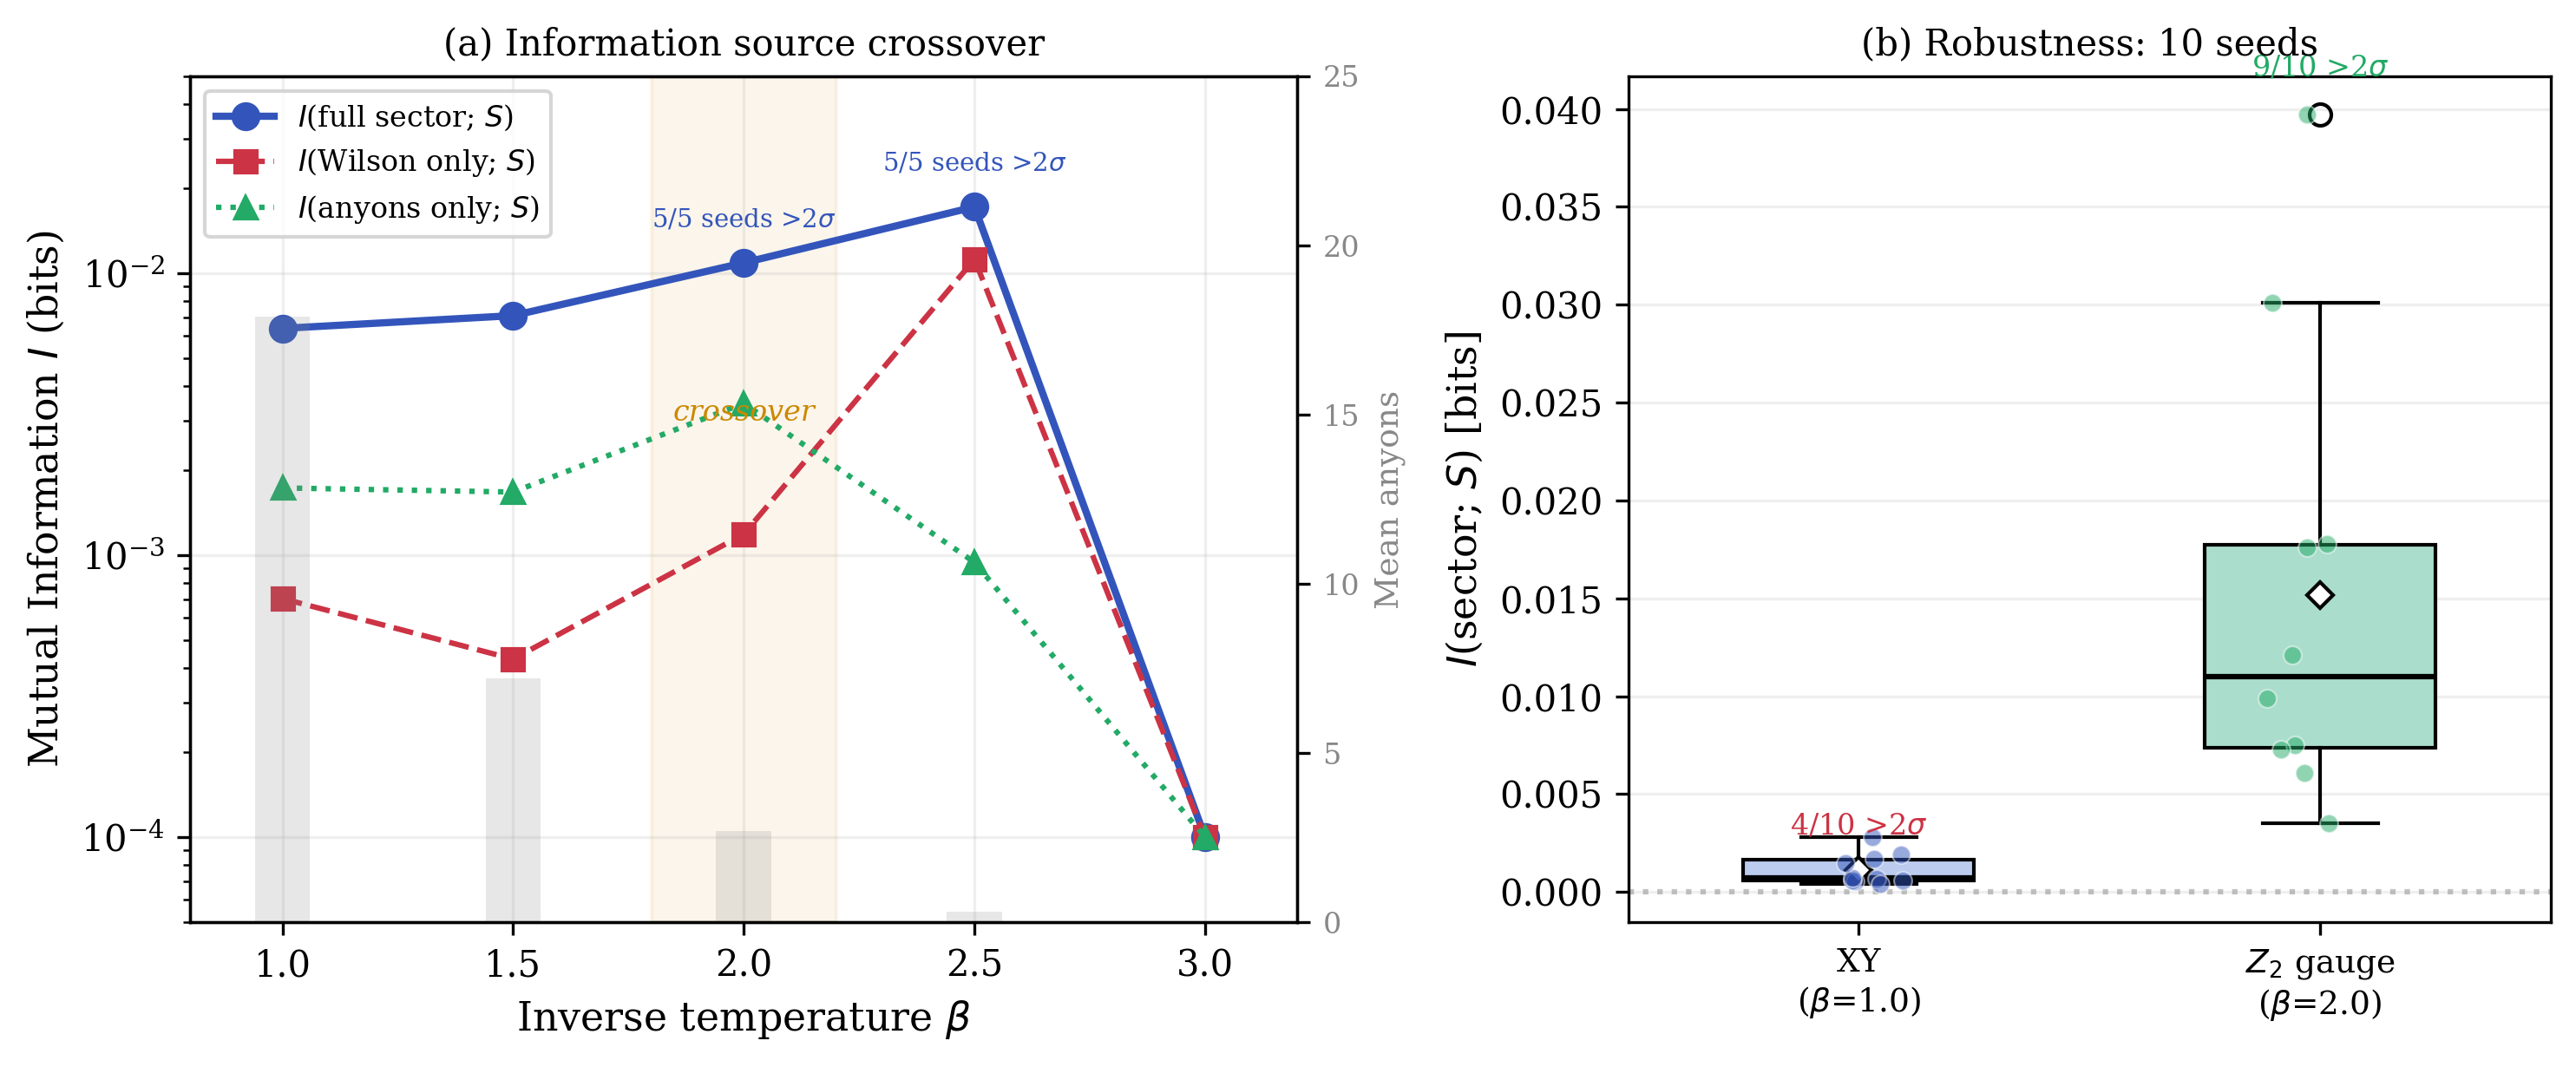
\includegraphics[width=\columnwidth]{figures/fig1_crossover_seeds.png}
  \caption{(a)~Mutual information vs.\ inverse temperature showing the crossover
  from anyonic to Wilson-loop information. Gray bars: mean anyon count.
  (b)~Seed variation: 10 independent runs per model. Values in (a) are
  clipped at $10^{-4}$ for the logarithmic axis; the $\beta = 3.0$ entries
  are identically zero (Table~\ref{tab:crossover}).}
  \label{fig:crossover}
\end{figure}

\subsection{Finite-Size Scaling of $\MI$}
\label{sec:z2_scaling}

\paragraph{Motivation.}
The $\MI = 0.015 \pm 0.011$~bits reported in the previous subsection is a
measurement at fixed lattice size $L=16$ and fixed temperature $\beta=2.0$.
A natural question, raised by gauge-theory generalities, is how this signal
scales with $L$: does it persist toward the thermodynamic limit, or is it a
finite-size effect of the $L=16$ system used for the original measurement? We
report here a dedicated scaling study at fixed $\beta=2.0$. The aim is not to
retract the $L=16$ value but to embed it in a scaling sequence.

\paragraph{Methods.}
We measure $\MI$ at $L \in \{8, 16, 32, 48, 64\}$, $\beta = 2.0$, with $10$
independent random-seed runs per $(L,\text{engine})$ cell. Two independent
Monte~Carlo engines are used, sharing the single-spin-flip Metropolis update
rule but differing in sweep order: (i)~the legacy engine
\texttt{z2\_sim\_v05.py} (same as for the $L=16$ primary result above)
sweeps the link variables in row-major order; (ii)~a newly written vectorized
engine \texttt{z2\_vec.py} updates the link variables in a checkerboard order.
The two engines are compared against the analytic single-plaquette expectation
$\langle B_p \rangle = \tanh(\beta)$ (Wegner duality limit, exact for the 2D
$\Ztwo$ gauge model at the level of single-plaquette averages). Statistical
significance per cell
is reported as $\sigma = (I_\mathrm{real} - \bar I_\mathrm{shuffled}) /
\mathrm{std}(I_\mathrm{shuffled})$ using $1000$ permutation shuffles, identical
to the protocol of Sec.~\ref{sec:results}. Three model classes are
pre-registered for the $L$-dependence fit: a pure power law $M_2 :
a L^{b}$; a power law with nonzero asymptote $M_{2c} : a L^{b} + c$; and a
constant-asymptote exponential $M_\mathrm{exp} : a e^{-b L} + c$. Model selection
is by Bayesian information criterion (BIC), with $\Delta\mathrm{BIC} > 6$ used
as the threshold for decisive preference among the three.

\paragraph{Results --- per-cell measurements.}
Table~\ref{tab:z2_scaling} reports $I_\mathrm{mean} \pm \mathrm{SEM}$ over the
10 seeds per cell, together with the standardized significance against the
permutation null. The legacy-engine value at $L=16$, $I = 0.0149 \pm 0.0036$~bits,
reproduces the $L=16$ primary result of Sec.~\ref{sec:results}
($0.015 \pm 0.011$~bits) to within $0.03\sigma$.

\begin{table}[b]
\caption{Mutual information $\MI$ vs.\ lattice size $L$ at fixed $\beta=2.0$,
two engines, 10 seeds per cell. $\sigma$ is the standardized deviation from
the permutation null (1000 shuffles per seed).}
\label{tab:z2_scaling}
\begin{ruledtabular}
\begin{tabular}{rcccc}
$L$ & v05: $I$ (bits) & $\sigma$ & vec: $I$ (bits) & $\sigma$ \\
\hline
 8 & $0.0372 \pm 0.0108$    & 3.5 & $0.0191 \pm 0.0029$     & 6.6 \\
16 & $0.0149 \pm 0.0036$    & 4.1 & $0.00694 \pm 0.00144$   & 5.1 \\
32 & $0.00235 \pm 0.00069$  & 2.5 & $0.000544 \pm 0.000628$ & 0.6 \\
48 & $0.000091 \pm 0.000315$ & 0.3 & $-3.5\!\times\!10^{-6} \pm 6.1\!\times\!10^{-5}$ & 0.2 \\
64 & $0.0000857 \pm 0.0000461$ & 0.6 & $2.9\!\times\!10^{-7} \pm 2.1\!\times\!10^{-5}$ & 0.5 \\
\end{tabular}
\end{ruledtabular}
\footnotetext{All cell-level values reproducible from
\texttt{data/stufe2\_analyse.json} (included in this release); seeds 10--19
systematic.}
\end{table}

\paragraph{BIC model comparison.}
Three model classes are pre-registered for the $L$-dependence of the
sector-shuffle-corrected $\MI(L)$ at $\beta=2.0$ (the raw $\MI$ minus the mean
$\MI$ of sector-shuffled surrogates, i.e., the permutation-null-subtracted
signal reported per cell in \texttt{data/stufe2\_analyse.json}): a pure power law
$M_2 : a L^{b}$ (2 parameters); a power law with nonzero asymptote
$M_{2c} : a L^{b} + c$ (3 parameters); and a constant-asymptote exponential
$M_\mathrm{exp} : a e^{-b L} + c$ (3 parameters). Table~\ref{tab:z2_bic}
reports BIC and $\chi^2$ for each model and each engine.

\begin{table}[b]
\caption{Bayesian information criterion (BIC) for three pre-registered
$L$-scaling models of $\MI(L)$ at $\beta=2.0$, fitted to
Tab.~\ref{tab:z2_scaling}. $\chi^2$ is the unweighted sum of squared
residuals. $\Delta\mathrm{BIC}_\mathrm{best\,vs\,2nd}$ above $6$ is the
pre-registered threshold for decisive preference; $2$--$6$ counts as positive
evidence.}
\label{tab:z2_bic}
\begin{ruledtabular}
\begin{tabular}{lrrrr}
Model & v05: BIC & v05: $\chi^2$ & vec: BIC & vec: $\chi^2$ \\
\hline
$M_2$                            & 12.33         & 9.11         & 15.77         & 12.55 \\
$M_{2c}$                         &  8.26         & 3.44         & 12.86         &  8.03 \\
$M_\mathrm{exp}$ (best)          & \textbf{5.11} & \textbf{0.28} & \textbf{5.69} & \textbf{0.86} \\
\hline
$\Delta\mathrm{BIC}_\mathrm{best\,vs\,2nd}$ & \multicolumn{2}{c}{3.15} & \multicolumn{2}{c}{7.18} \\
\end{tabular}
\end{ruledtabular}
\footnotetext{Fit parameters and per-$L$ predictions reproducible from
\texttt{data/stufe2\_analyse.json}.}
\end{table}

\paragraph{Engine consensus.}
$M_\mathrm{exp}$ minimizes BIC in both engines (Fig.~\ref{fig:z2_scaling}). The strength of the preference
differs: in the vectorized engine
$\Delta\mathrm{BIC}_\mathrm{best\,vs\,2nd} = 7.18$, above the pre-registered
decisive threshold; in the legacy engine the gap is $3.15$, positive but
sub-decisive. Given the sub-decisive gap in the legacy engine, the
engine-consensus carries the model-selection conclusion, not either engine
alone --- $M_\mathrm{exp}$ is the \emph{preferred} model among the
pre-registered set, not a uniquely determined one. The fitted exponential rate
is consistent across engines: $b = 0.125 \pm 0.020$ (v05) and
$b = 0.140 \pm 0.024$ (vec), corresponding to a characteristic length scale of
$1/b \approx 7$--$8$ lattice spacings. The fitted asymptote $c$ is statistically
indistinguishable from zero in both engines:
$c = (0.62 \pm 8.8) \times 10^{-5}$ (v05) and
$c = (0.10 \pm 3.2) \times 10^{-5}$ (vec), each with
$|c|/\mathrm{SEM}(c) < 0.1$. Two qualitative conclusions follow that are
robust across both engines: (i)~$\MI(L)$ decays faster than any power law
in the tested range, and (ii)~the asymptote is data-supported (not
extrapolated) to be indistinguishable from zero. The absolute $L=16$ value
is, however, \emph{not} engine-robust --- see disclosure below.

\paragraph{v05 engine-specific bias --- disclosure.}
The two engines do not agree on the absolute $\MI$ value at fixed $(L,\beta)$.
At $L=16$, $\beta=2.0$, the legacy engine reports $I = 0.0149 \pm 0.0036$~bits
while the vectorized engine reports $I = 0.00694 \pm 0.00144$~bits, a factor of
$\sim 2.15$. The two engines also differ in their reproduction of the analytic
single-plaquette expectation $\langle B_p \rangle = \tanh(\beta)$
(Wegner-duality limit, exact for the 2D~$\Ztwo$ gauge model at the level of
single-plaquette averages): at $\beta=2.0$ the vectorized engine matches the
analytic value to $0.1\%$, while the legacy engine deviates by $+2.2\%$
toward colder configurations. This diagnostic
\emph{identifies} the bias as present; its precise mechanism has not been
isolated by a dedicated thermalization-scaling run. The deviation is
\emph{consistent with} the legacy engine's row-major sweep order, which
(compared to the vectorized checkerboard-sweep engine of identical
Metropolis-update rule) is expected to require longer thermalization to
reach detailed-balance equilibrium, and/or with initial-state-dependent
trapping in the ordered basin; the diagnostic data do not select among these
candidate mechanisms. The diagnostic also does not, by itself, \emph{select} among the
three scaling models above; model selection rests on the BIC comparison of
Tab.~\ref{tab:z2_bic}. The previously reported $I = 0.015 \pm 0.011$~bits at
$L=16$ (Sec.~\ref{sec:results}) is, accordingly, \emph{not retracted}: it
remains a correct measurement of the legacy engine's output. Its absolute
numerical value is, however, to be read as engine-specific rather than as an
engine-independent quantity. Both qualitative conclusions of the consensus
paragraph above --- faster-than-power-law decay and vanishing asymptote ---
survive the engine-specificity.

\begin{figure}[t]
  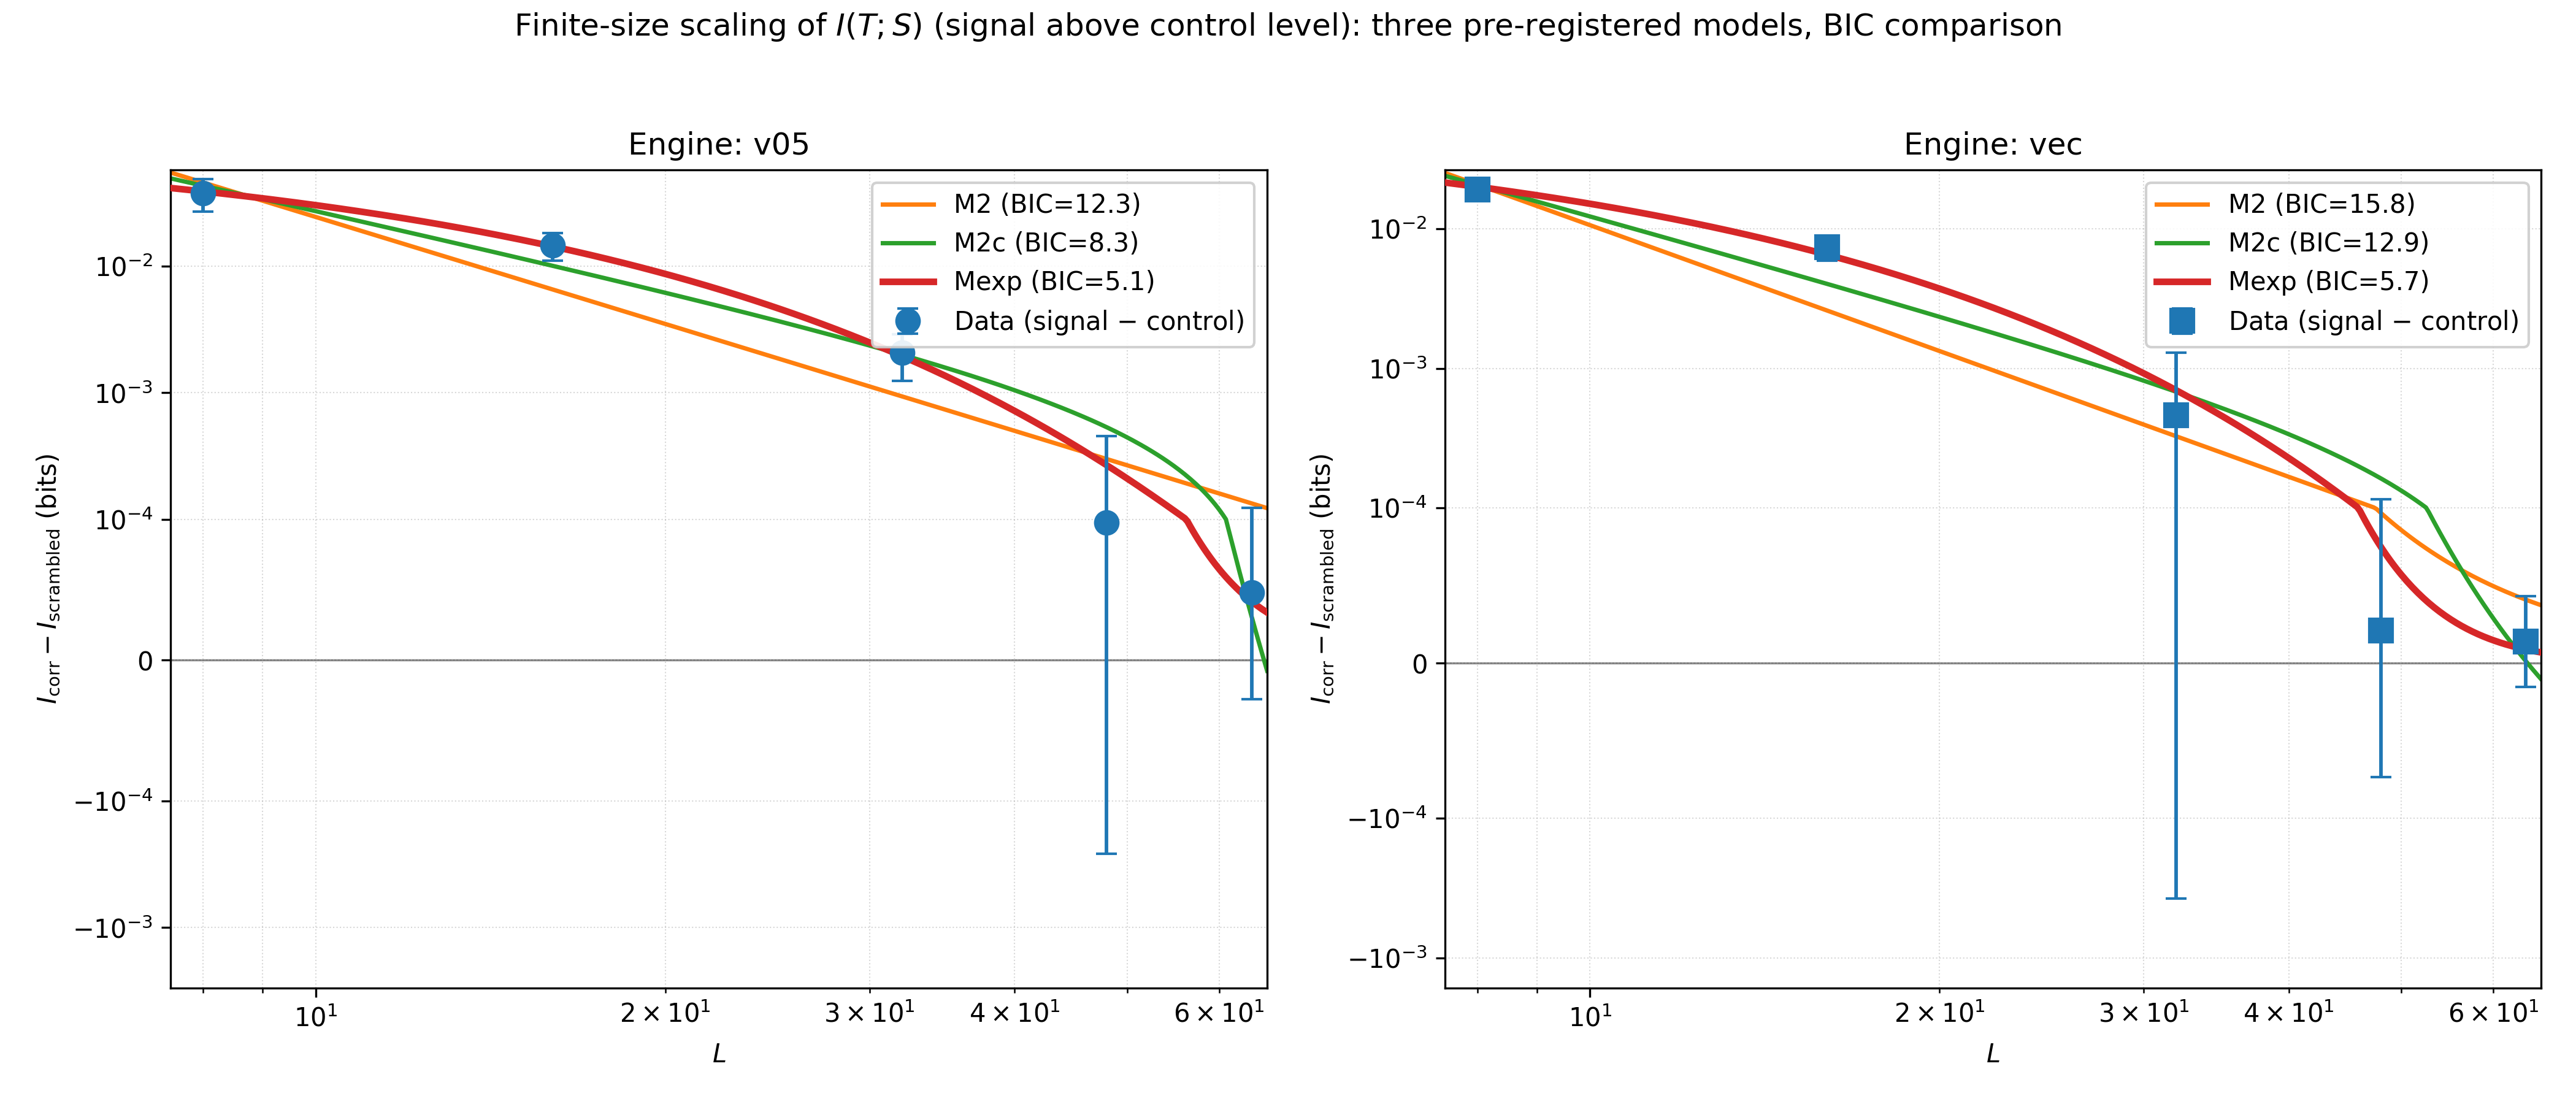
\includegraphics[width=\columnwidth]{figures/fig4_z2_scaling.png}
  \caption{Finite-size scaling of $\MI$ in 2D $\Ztwo$ gauge theory at
  $\beta=2.0$. Per-cell measurements (Tab.~\ref{tab:z2_scaling}) with two
  Monte-Carlo engines (legacy v05 = circles, vectorized vec = squares) and
  the three pre-registered fit curves (Tab.~\ref{tab:z2_bic}): pure power
  $M_2$, power-with-asymptote $M_{2c}$, exponential $M_\mathrm{exp}$.
  $M_\mathrm{exp}$ is the BIC-preferred model in both engines (decisive in
  vec, sub-decisive in v05). The engine-consensus conclusion is qualitative:
  $\MI(L)$ decays faster than any power law, with asymptote data-supported
  to be zero within the measurement precision. The absolute $L=16$ value is
  engine-specific (see disclosure in text).}
  \label{fig:z2_scaling}
\end{figure}

\paragraph{Conclusion.}
The subsection has two robust takeaways and one scope-limiting statement.
\emph{Robust:} (i)~at fixed $\beta=2.0$, $\MI(L)$ decreases faster than any
power law in the tested range $L \in \{8,16,32,48,64\}$, with the
exponential form $M_\mathrm{exp}$ preferred under the pre-registered set in
both engines; (ii)~the asymptote is data-supported (not extrapolated) to be
statistically indistinguishable from zero. \emph{Engine-specific:} the
absolute $L=16$ value differs by a factor of $\sim 2$ between the two
engines and should be read as engine-specific (legacy: $0.0149$~bits,
vectorized: $0.00694$~bits); the qualitative trend is unaffected by this
specificity. \emph{Scope.} The methodological question of how a
finite-size $\MI > 0$ at $L=16$ that decays toward zero at larger $L$
should be interpreted --- in particular, whether the observed signal admits
a non-finite-size physical reading --- is beyond the empirical scope of this
paper and is deferred to future theoretical work.

\subsection{XY Model: Exploratory}

In the XY model at $\beta = 1.0$, seed variation reveals that $I(|n|;\,S)$ is not
robust: only 4/10 runs exceed $2\sigma$ (2/10 ${>}3\sigma$). Mean:
$I = 0.001 \pm 0.001$~bits at $1.5 \pm 1.9\,\sigma$. The trend
$\uparrow|n| \to \downarrow S$ has correlation $r = +0.03 \pm 0.75$, consistent
with zero. We report this as exploratory. The signal may require larger lattices
or longer runs to establish in this noisier model.

Vortex-antivortex correlations show Coulomb-like attraction ($g(r{=}1) = -0.78$)
consistent with BKT physics~\cite{KT1973}, and the CHSH value anti-correlates
with defect count ($r = -0.90$), indicating that topological disorder degrades
CHSH correlations.

\subsection{Quantum Toric Code}

At $L = 2$ (8~qubits), $m$-anyon pairs yield $|S| = \sqrt{2}$ with the sign
flipping between sectors ($I = 0.350$~bits, $1595\sigma$). At $L = 3$
(18~qubits), all single-qubit and Wilson-loop correlations are exactly zero ---
verified across all 153 qubit pairs and all operator types
($\sigma^z$-$\sigma^z$, $\sigma^x$-$\sigma^x$, mixed).

The $L = 2$ result is a finite-size artifact: on a $2 \times 2$ torus,
measurement qubits simultaneously belong to the string, the plaquettes, and
noncontractible loops. At $L \geq 3$, the abelian nature of $\Ztwo$ anyons means
their entanglement is encoded globally and cannot be accessed by any operator that
is a product of Pauli matrices on a subset of edges~\cite{Wen2002,Nayak2008}.

\subsection{Systematic Negative Results}

We tested three classical mechanisms for Bell violation beyond the Fine
bound~\cite{Fine1982}:

\textbf{(i)~Measurement-rule modification:} Making $A(a, \lambda)$ depend on the
topological sector~$n$ via a phase shift
$A = \mathrm{sign}(\cos(a - \theta + n\alpha))$ \emph{decreases} $|S|$ --- the
coupling adds noise rather than correlation.

\textbf{(ii)~Statistical-independence violation:} Weighting configurations by
$\rho(n|a,b)$ allows $S$ to reach 2.000 exactly but never exceed it. Fine's theorem
guarantees $|S| \leq 2$ for deterministic local functions $A(a, \lambda)$ and
$B(b, \lambda)$ only when the hidden-variable weighting $\rho(\lambda)$ is
\emph{setting-independent}; the present family $\rho(n|a,b)$ is explicitly
setting-dependent, so the theorem's hypothesis is not strictly satisfied here. Our
result is narrower and empirical: this particular sector-mediated weighting family
caps at $S=2.000$ in the numerics tested, not a general re-derivation of the Fine
bound for setting-dependent weightings.

\textbf{(iii)~Transport phase:} Including a gauge-field phase accumulated along
the path between detectors produces the correct angular form (correlation with
$-\cos\theta$ at $r = 0.993$) but only 17\% of the quantum-mechanical amplitude.
Thermal fluctuations wash out the phase coherence.

\begin{figure}[t]
  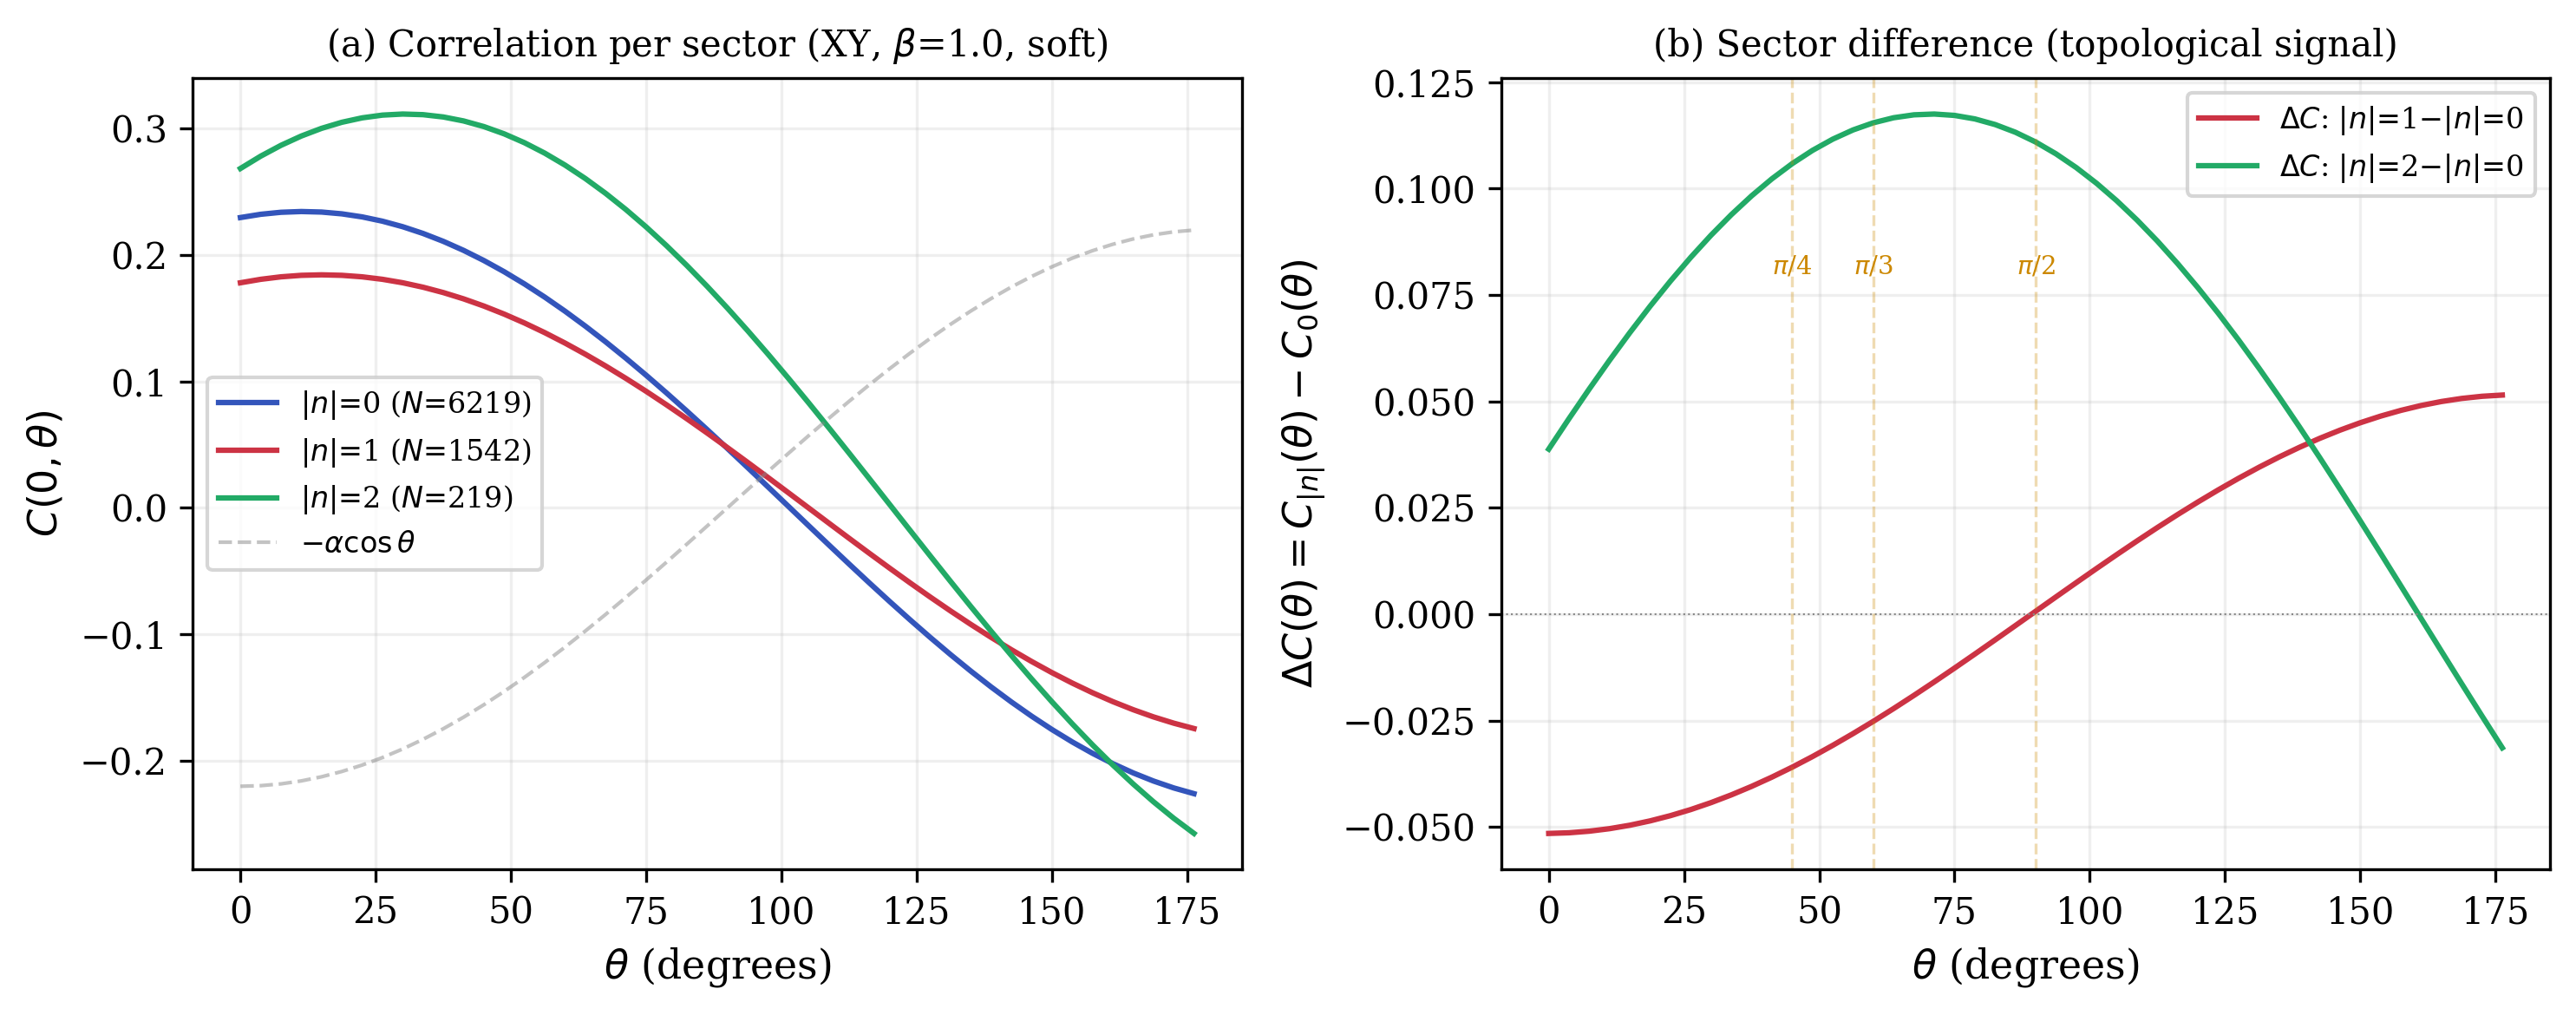
\includegraphics[width=\columnwidth]{figures/fig2_sector_correlation.png}
  \caption{(a)~Correlation $C(0, \theta)$ per winding-number sector in the XY
  model (soft measurement). (b)~Sector difference
  $\Delta C = C_{|n|}(\theta) - C_0(\theta)$, isolating the topological signal.
  Dashed lines mark predicted resonance angles $\pi/n$.}
  \label{fig:sector_corr}
\end{figure}

\subsection{Fourier Analysis}

The sector difference $\Delta C(\theta)$ (Fig.~\ref{fig:sector_corr}) shows the dominant Fourier mode is
$k = 1$ in all sectors, inconsistent with the prediction that the mode should
scale with winding number~$n$. A weak resonance enhancement at $\theta = \pi/n$
for $|n| \geq 2$ (amplitude ratio 1.20--1.38) is observed but not statistically
decisive. The even-harmonic structure in raw residuals ($a_2 \gg a_1$) is an
artifact of the $\mathrm{sign}(\cos)$ measurement discretization, eliminated by
using soft ($\cos$) measurements.

\subsection{Fibonacci Anyons: CHSH Violation}
\label{sec:fibonacci}

Fibonacci anyons have fusion rule $\tau \times \tau = 1 + \tau$ (golden ratio
quantum dimension) and no fermion parity superselection. Their braiding generates
a dense subset of $\mathrm{SU}(2)$ per logical qubit, making them universal
for quantum computation~\cite{Freedman2003}. We simulate the fusion space of
six Fibonacci anyons (two logical qubits) with braid gates constructed from the
Fibonacci
$F$-matrix
\begin{equation}
  F = \begin{pmatrix} \varphi^{-1} & \varphi^{-1/2} \\
  \varphi^{-1/2} & -\varphi^{-1} \end{pmatrix},
  \quad \varphi = \tfrac{1+\sqrt{5}}{2},
  \label{eq:fib_f_matrix}
\end{equation}
and $R$-matrix ($R_1 = e^{-4i\pi/5}$, $R_\tau = e^{3i\pi/5}$).

Table~\ref{tab:fibonacci} shows the CHSH value as a function of braiding sequence
length. All enumerated sequences from $L=3$ to $L=12$ violate the classical
CHSH bound $|S|>2$, with $|S|$ rising monotonically from $2.199$ at $L=3$ to
$|S|=2.811$ at $L=12$ ($99.4\%$ of the Tsirelson bound $2\sqrt{2}$, $C=0.988$).
These $|S|$ values are signatures of topological nonseparability on the
nonfactorized Fibonacci fusion space, not Bell violations in the
Einstein--Podolsky--Rosen bipartite sense.
The optimal length-12 sequence is
$(\sigma_1\sigma_2)^6$,
where $\sigma_1$ braids the Alice--mediator pair and $\sigma_2$ braids the
mediator--Bob pair. This result is exact within the TQFT description of Fibonacci
anyons and was obtained by full enumeration over all $2^L$ sequences combined
with the Horodecki bound $|S|_{\max} = 2\sqrt{1+C^2}$~\cite{Horodecki1995}, as
detailed in the companion paper Ref.~\cite{Sayim2026fibonacci}; see
\textit{Note on optimization} below for the v2.0 $\to$ v2.1 correction.


\begin{table}[b]
\caption{Fibonacci anyon CHSH violation vs.\ braiding sequence length
(values reproduced from Ref.~\cite{Sayim2026fibonacci} Tab.~I via full enumeration
over all $2^L$ sequences and 50 sector-phase values; Horodecki bound
$|S|_{\max} = 2\sqrt{1+C^2}$~\cite{Horodecki1995} from the maximal
concurrence~$C$).  Sequence notation: $A = \sigma_1$ (Alice--mediator braid),
$B = \sigma_2$ (mediator--Bob braid).}
\label{tab:fibonacci}
\begin{ruledtabular}
\begin{tabular}{rcccc}
$L$ & $|S|$ & $C$ & \% Tsirelson & Sequence \\
\hline
 3 & 2.199 & 0.457 & 77.7 & ABB \\
 4 & 2.225 & 0.488 & 78.7 & ABAB \\
 5 & 2.348 & 0.615 & 83.0 & AABAB \\
 6 & 2.398 & 0.662 & 84.8 & ABBAAB \\
 7 & 2.536 & 0.780 & 89.7 & ABBAABB \\
 8 & 2.540 & 0.783 & 89.8 & BABBABAB \\
 9 & 2.624 & 0.850 & 92.8 & ABBAABABB \\
10 & 2.696 & 0.904 & 95.3 & ABBAABBAAB \\
11 & 2.784 & 0.968 & 98.4 & ABABBBBABAB \\
12 & \textbf{2.811} & \textbf{0.988} & \textbf{99.4} & \textbf{ABABABABABAB} \\
\end{tabular}
\end{ruledtabular}
\footnotetext{The original v2.0 table reported lower $|S|$ values for
$L \leq 11$ from an X-Z-restricted angular optimizer; these have been replaced
in v2.1 by the Horodecki-bound full enumeration of Ref.~\cite{Sayim2026fibonacci}.  See
\textit{Note on optimization} below for the correction trail.}
\end{table}

Critically, the violation is strongly sector-dependent. When the topological
sector phase~$\delta$ is varied (modifying the relative phase between fusion
channels), the concurrence ranges from $0$ to $0.99$ over the
$\delta\in[0,2\pi)$ sweep ($N=200$ points). Throughout this Fibonacci sweep,
$\delta$ should be read as a representation-deformation parameter rather than
a physical anyon parameter: as verified numerically in the companion landscape
analysis [\cite{Sayim2026fibonacci}, Appendix~C], generic $\delta\neq0$ breaks
the Yang--Baxter/hexagon consistency of the braid representation, and only
$\delta=0$ realizes the standard Fibonacci modular tensor category. With \emph{fixed} measurement
settings (optimized at the winner sector $\delta\approx 1.44\pi$), $|S|$ ranges
from near zero (when settings are misaligned with the sector basis) to
$2.72$, with CHSH violation observed in $14\%$ of sectors.
When measurement settings are instead optimized per-sector via the full
Bloch-sphere parametrization (the same methodology used in
Table~\ref{tab:fibonacci}), the per-sector maximum reaches $|S|=2.811$
at $\delta\approx 1.76\pi$ --- the same Bloch optimum that defines the
Table~\ref{tab:fibonacci} winning value at $L=12$.
With \emph{adapted}
settings via the Horodecki bound, $|S|$ ranges from $2.000$ to $2.811$, and
CHSH violation is achieved in $99.5\%$ of sectors. Different sectors thus
require different detector calibrations for maximum violation. This is
consistent with the central interpretive claim of this work: \textbf{topology
is consistent with neither creating nor destroying entanglement, but rotating
the optimal measurement basis in fusion space.} (The entanglement itself, as
measured by concurrence, does vary substantially with sector --- from $0$ to
$0.99$ over the $\delta$-sweep above --- so this claim is scoped to the
CHSH-violation ceiling under adapted settings, not to sector-invariance of the
entanglement.)

Unlike Ising anyons (Sec.~\ref{sec:ising_prediction}), Fibonacci anyons have no
fermion parity restriction on local measurements. The full Pauli algebra is
accessible in the fusion space, enabling CHSH-form violation with local
braid-then-fuse operations on the fusion space. This resolves the $S = 2.000$ saturation
observed for Ising anyons and establishes Fibonacci anyons as the minimal model
for topological CHSH violation among the models tested here.

\paragraph{Note on optimization (added 2026-04-15, extended 2026-05-28).}
The length-12 value $|S| = 2.811$ reported here supersedes an earlier estimate
$|S| = 2.554$ obtained from the original angle-search optimizer (six random
seeds plus a $9^4$ grid). A subsequent full enumeration of winning sequences,
combined with the analytic Horodecki bound
$|S|_{\max} = 2\sqrt{1+C^2}$~\cite{Horodecki1995}, recovers $|S| = 2.811$ at
$C = 0.988$ for the optimal length-12 sequence $(\sigma_1\sigma_2)^6$
($99.4\%$ of the Tsirelson bound).
The earlier value is therefore an optimization artifact, not a physical limit.
The same enumeration shows that both encodings considered for the six-Fibonacci
fusion space (the two-generator d1b encoding used here and the three-generator
encoding on the full $5$-dimensional fusion space) are dense in $\mathrm{SU}(4)$
and, under standard four-dimensional computational-subspace measurement,
reach comparable CHSH values near the Tsirelson bound; they differ primarily
in the minimum word length required ($L \approx 12$ vs.\ $L \approx 8$).
Protocol-dependent differences --- in particular the gap between native-$5$D
CHSH and the $4$D-projected value, and the associated leakage statistics ---
are documented in the companion paper
Ref.~\cite{Sayim2026fibonacci}.

\smallskip
\textit{v2.1 update (2026-05-28).}
The same Horodecki-bound full enumeration has been applied to lengths
$L = 3$--$11$ in v2.1, replacing the original X-Z-plane restricted angular
optimizer used in v2.0 (and earlier versions) for those rows of
Tab.~\ref{tab:fibonacci}.  The restricted optimizer reported systematically
lower values (mean deficit ${-}0.60$, maximum ${-}1.04$ at $L = 3$) and
suboptimal winning sequences, because complex-phase $R$-matrices in the Fibonacci
braid representation require measurement operators rotated outside the X-Z
plane to saturate the Horodecki maximum.  With the corrected values, the trend
is monotonic in both $|S|$ and $C$ from $L=3$ to $L=12$; the earlier
"nonmonotonicity" interpretation in v2.0 was therefore an optimizer artifact
and has been removed.  See Ref.~\cite{Sayim2026fibonacci} Tab.~I for the underlying
enumeration.

\section{Discussion}
\label{sec:discussion}

\subsection{Summary of Established Results}

We establish three main results at increasing levels of significance. First,
topological sectors and CHSH values are not statistically independent in the
$\Ztwo$ lattice gauge theory at $\beta = 2.0$ ($I = 0.015 \pm 0.011$~bits, 9/10
seeds ${>}2\sigma$, confirmed gauge-invariant at 21/21 ${>}3\sigma$); the
crossover decomposition of Table~\ref{tab:crossover} shows that at this
coupling the signal is carried by the anyonic (local-defect) component of the
sector label (significant in 3 of 5 validation seeds), while the genuinely
topological Wilson-loop component remains below significance (1 of 5); and this
mutual-information signal is, moreover, a finite-size effect that decays toward
zero with system size (Sec.~\ref{sec:z2_scaling}). Second, an
information-source crossover from defect-mediated to sector-mediated correlation
occurs near $\beta \sim 2.0$ --- a new observation, to our knowledge, in this
specific information-theoretic context. Third, and most significantly,
Fibonacci anyon braiding produces CHSH violation with $|S| = 2.811$ ($99.4\%$
Tsirelson), and this violation is strongly sector-dependent: with fixed
detector settings, $|S|$ varies from near zero to $2.72$ across the topological
sector phase $\delta \in [0, 2\pi)$.

The Fibonacci result resolves the hierarchy of negative results: $\Ztwo$ classical
models cannot violate Bell (Fine's theorem), abelian quantum anyons are locally
invisible ($L \geq 3$ toric code), and Ising anyons saturate at $S = 2.000$
(fermion parity). Fibonacci anyons, with no parity restriction and universal
braiding, are the minimal model that achieves topological CHSH violation among
the models tested here.

\subsection{Limitations}

All results reported here are numerical simulations within idealized TQFT
models, not laboratory experiments.
The Fibonacci CHSH violation is computed in the ideal TQFT fusion space --- a
unitary, zero-temperature, zero-decoherence model. In a physical realization
(e.g., $\nu = 12/5$ fractional quantum Hall state), thermal excitations, finite
system size, and quasiparticle tunneling would reduce $|S|$ below the ideal value.
The $\Ztwo$ results, while robust, show $I \sim 0.01$--$0.04$~bits --- a small
effect. The XY model result is not robust across seeds. The elevated mutual
information at $\beta = 2.5$ reflects the near-frozen anyon sector of the anchor
engine, in which the sector label collapses onto its Wilson-loop component, not
a nontrivial topological mechanism.

\subsection{Implications for Topological Interpretations}

The Fibonacci result is consistent with non-Abelian topological order producing
sector-dependent CHSH violation with strictly local measurements. This means:
(i)~the topological sector acts as a classical degree of freedom that modulates measurement
correlations, (ii)~the modulation is strong enough to cross the classical bound, and
(iii)~an observer who does not know the sector sees reduced $|S|$ on average ---
the topology \emph{obscures} the violation rather than creating it --- a property
of the idealized topological order itself, independent of any interpretation of
the measurement process.

\subsection{Prediction: Sector-Dependent CHSH Violation in Non-Abelian Models}
\label{sec:ising_prediction}

We present an analytical argument that non-Abelian topological order produces
sector-dependent CHSH correlations. For Ising anyons, the braiding $R$-matrix has
two eigenvalues corresponding to the two fusion channels~\cite{Nayak2008,Kitaev2006}:
\begin{equation}
  R_1 = e^{-i\pi/8}, \qquad R_\psi = e^{3i\pi/8}.
  \label{eq:ising_r}
\end{equation}
On a torus, the topological sector modifies the relative phase between these
channels. In sector~$\delta$, the $R$-matrix becomes
$R_1 = e^{-i\pi/8}$, $R_\psi = e^{i(3\pi/8 + \delta)}$, where $\delta$ depends
on the anyon type threading the noncontractible loop~\cite{Kitaev2003,Kitaev2006}.
Here $\delta$ is a physical sector phase fixed by the threading anyon --- a
discrete, topologically determined label --- rather than a freely tunable
deformation parameter.
Braiding two pairs of Ising anyons produces the entangled fusion state:
\begin{equation}
  \ket{\psi(\delta)} = \cos\alpha\,\ket{00} + e^{i\delta}\sin\alpha\,\ket{11},
  \label{eq:ising_state}
\end{equation}
where $\alpha$ is determined by the braiding sequence and $\ket{0}$, $\ket{1}$
label the fusion channels (vacuum and fermion respectively). For maximal braiding
($\alpha = \pi/4$), the concurrence is 1 for all~$\delta$ --- the entanglement is
sector-independent. However, the CHSH value with \emph{fixed} measurement settings
is strongly sector-dependent:
\begin{equation}
  S(\delta) = 2\sqrt{2}\,\cos^2(\delta/2)
  \qquad\text{(settings optimized at $\delta{=}0$)}.
  \label{eq:s_delta}
\end{equation}

We verify this numerically: with settings optimized for the vacuum sector
($\delta = 0$), $S$ ranges from $2\sqrt{2} \approx 2.83$ (maximal CHSH violation)
at $\delta = 0$ to $S = \sqrt{2} \approx 1.41$ at $\delta = \pi/2$, and $S = 0$
at $\delta = \pi$, following the $\cos^2(\delta/2)$ law. Critically:

(i)~\textbf{CHSH violation is preserved in all sectors} if measurement settings
are adapted --- $\max|S| = 2\sqrt{2}$ for all~$\delta$. The topology does not
create or destroy entanglement.

(ii)~\textbf{With fixed settings, $S$ depends on the sector} --- producing
$\MI > 0$. This is the non-Abelian analogue of our $\Ztwo$ result, but now with
actual CHSH violation.

(iii)~\textbf{The sector rotates the optimal measurement basis} in the fusion
space. Different sectors require different detector calibrations to see maximum
violation. An observer who does not know the sector sees reduced~$S$ on average.

This constitutes a concrete analytical prediction, subject to the parity caveat
below: in any experiment that
creates and braids Ising anyons on a surface with nontrivial topology, the
observed CHSH value must depend on the topological sector. The functional form ---
$\cos$-modulation with period determined by the anyon type threading the handle
--- is parameter-free.

\textbf{Caveat:} Numerical verification via a Majorana fermion representation
shows that the braid-then-fuse measurement protocol saturates at $S = 2.000$
exactly for Ising anyons, due to the fermion parity superselection rule:
Pauli-$X$ operators project to zero in the even-parity sector, restricting local
measurements to the $Z$-basis. This limits Ising anyons to the classical bound with
strictly local measurements~\cite{HowardVala2012}. The prediction
$S(\delta) = 2\sqrt{2}\cos^2(\delta/2)$ applies when measurements in the full
fusion-space basis are available, as would be the case for Fibonacci anyons where
no parity restriction exists. Fibonacci anyons are therefore the natural target for
experimental verification. A companion paper~\cite{Sayim2026cbell}
constructs this noncommuting CHSH operator algebra locally in the Kitaev
honeycomb model; as noted above, a genuine violation with topologically
protected Ising operations requires nonstabilizer (magic) resources.

\subsection{Related Work and Prior Art}
\label{sec:related_work}

The CHSH-violation construction presented here for Fibonacci anyons sits in
a broader landscape of topological and nonstandard Bell tests. Earlier
qualitative Bell-test constructions for non-Abelian anyons were proposed by
Brennen, Iblisdir, Pachos, and Slingerland~\cite{Brennen2009} for Fibonacci
and Ising anyons; Chang, Chu, and Ma~\cite{ChangChuMa2017} studied Bell's
inequality in topologically ordered qubit models (Wen-plaquette). On Majorana
platforms, Drummond, Kovalev, Hou, Shtengel, and Pryadko~\cite{Drummond2014}
gave an explicit CHSH protocol for Majorana wires, and Romito and
Gefen~\cite{RomitoGefen2017} demonstrated nonlocal entanglement with six
Majorana zero modes reaching the Tsirelson bound. Single-particle Bell-like
inequality violations in neutron interferometry were reported by
Hasegawa, Loidl, Badurek, Baron, and
Rauch~\cite{Hasegawa2003}; the contextuality-based program of
Liu, Hu, Chen, Huang, Han, Li, Guo, and
Cabello~\cite{Liu2016Cabello} provides a complementary view on the relation
between nonlocality and contextuality. The present paper differs from these
works in scope: we report the mutual-information structure $I(T;S)$ between
topological sectors and CHSH values across a hierarchy of lattice and anyonic
models, including the finite-size scaling reported in
Sec.~\ref{sec:z2_scaling}, rather than a single Bell-test protocol on a fixed
topological platform.

Independently and contemporaneously, Xu, Ye, and You~\cite{Xu2025} have
studied CHSH correlations on Fibonacci anyonic states using a three-copy
fusion-sector observables construction (their Eq.~(9)), reporting
$|S| \approx 2.633$ on $|\tau,\tau;1\rangle^{\otimes 3}$. Their setup differs
from ours in both the ambient fusion space and the observable choice; a
detailed setup-by-setup comparison appears in the companion
paper~\cite{Sayim2026fibonacci}.

Recent methodological work on braid-circuit verification by
Amaral~\cite{Amaral2025} and on minimal-depth Levin--Wen circuits by
Bseiso \emph{et al.}~\cite{Bseiso2024} provides additional methodological
context for the F-symbol conventions and Yang--Baxter checks used here. A
companion Leggett--Garg-inequality analysis on the same Fibonacci representation,
saturating the L\"uders bound $K_3 \to 3/2$, is reported separately in
Ref.~\cite{Sayim2026LGI}.

\subsection{Relation to Companion Work and Open Questions}

Two of the directions previously listed here have in fact already been carried
out and are reported elsewhere. The convergence of $|S|$ toward the Tsirelson
bound and the complete braid landscape for lengths beyond $L=12$ are analyzed in
the companion paper Ref.~\cite{Sayim2026fibonacci}; the temporal-correlation
counterpart on the same Fibonacci representation, using Leggett--Garg-style
protocols, is reported in Ref.~\cite{Sayim2026LGI}. The finite-size scaling of
the $\Ztwo$ sector--CHSH mutual information is settled within the present paper
(Sec.~\ref{sec:z2_scaling}), where it is shown to decay toward zero with system
size. Two questions remain genuinely open. Whether a microscopic Hamiltonian
realization --- for example the Kitaev honeycomb model in its non-Abelian
phase~\cite{Kitaev2006} --- reproduces the idealized-TQFT sector dependence is
not established here. And whether the sector-dependence generalizes to other
non-Abelian anyon models, such as $\mathrm{SU}(2)_k$ theories at level
$k \geq 3$, is likewise not addressed by the present construction.

\begin{figure}[t]
  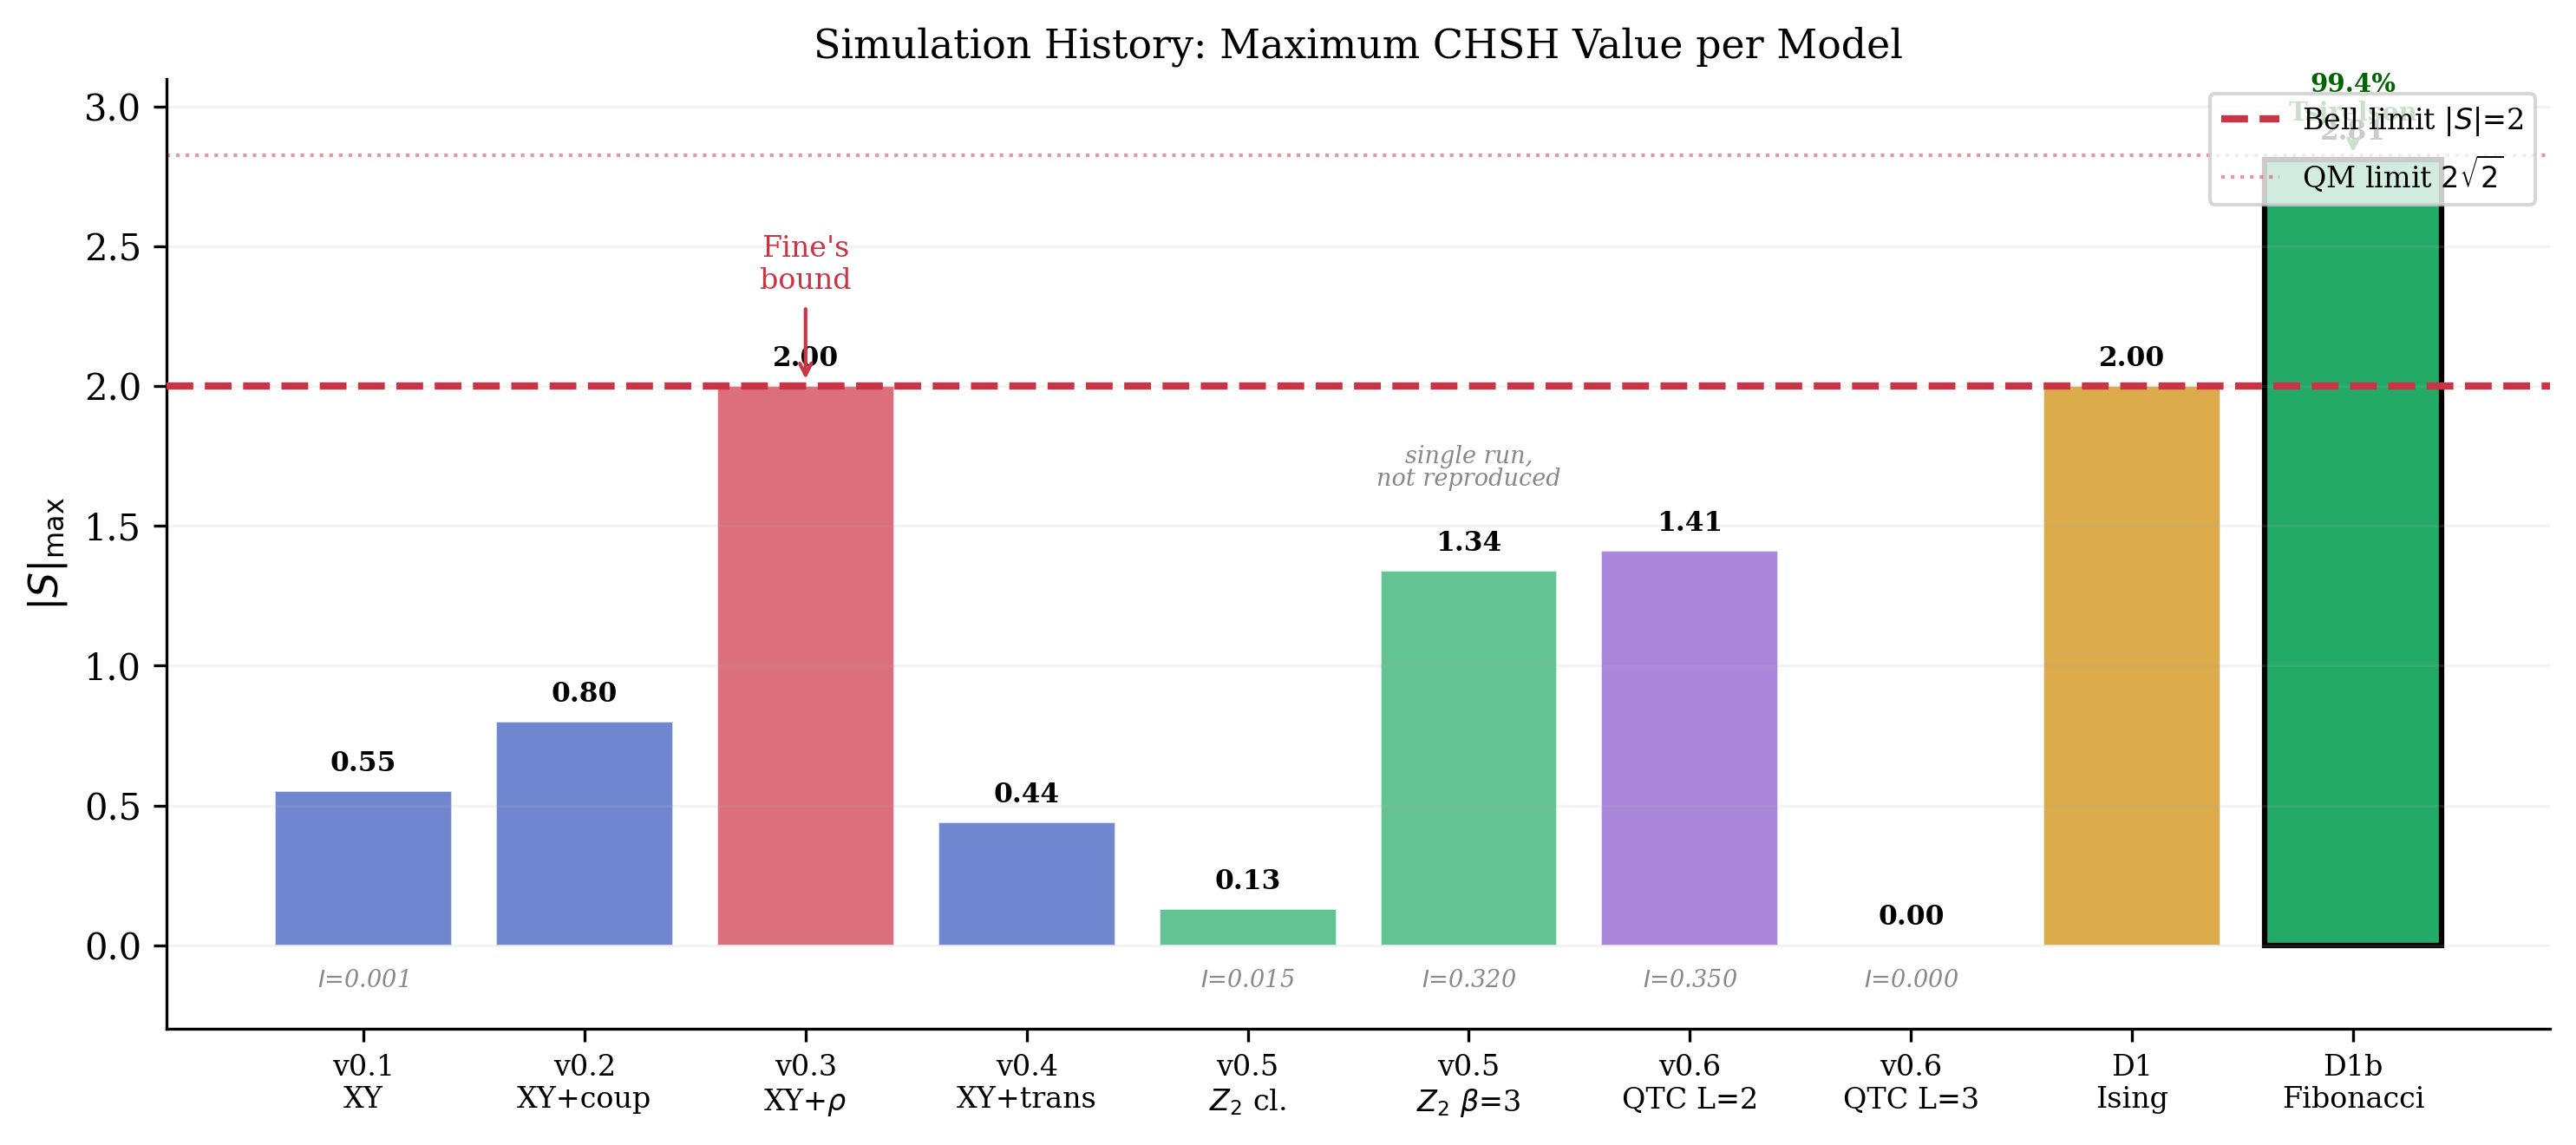
\includegraphics[width=\columnwidth]{figures/fig3_overview.png}
  \caption{Maximum CHSH value across all simulation models. The classical limit
  $|S| = 2$ (dashed red) is never exceeded in abelian models. Fibonacci anyons
  at braiding length~12 achieve $|S| = 2.811$ ($99.4\%$ of the Tsirelson bound
  $2\sqrt{2}$; corrected value, see Note on optimization, Sec.~\ref{sec:fibonacci}).}
  \label{fig:overview}
\end{figure}

\section{Conclusion}
\label{sec:conclusion}

We have presented a systematic numerical investigation demonstrating that topological structure produces
sector-dependent CHSH violation in a non-Abelian anyon model. The progression from
classical $\Ztwo$ gauge theory ($\MI > 0$, 9/10 seeds ${>}2\sigma$) through
abelian quantum anyons (locally invisible at $L \geq 3$) to Fibonacci anyons
($|S| = 2.811$, sector-dependent) traces a clear path: only non-Abelian
topological order with universal braiding generates CHSH violation through
topology in the models tested here (Fig.~\ref{fig:overview}).

The key finding is consistent with the topological sector neither creating nor
destroying entanglement, but rotating the optimal measurement basis in fusion
space --- scoped to the CHSH-violation ceiling under adapted settings, since
the entanglement itself (concurrence) varies substantially with sector, from
$0$ to $0.99$ over the Fibonacci $\delta$-sweep (Sec.~\ref{sec:fibonacci}). An
observer who does not know the sector sees variable $|S|$, ranging from near
zero to $2.72$ with fixed settings. This mechanism --- topology as a structured
classical degree of freedom that modulates which correlations are visible ---
provides a concrete analytical framework connecting topological order to the
structure of quantum correlations. The $\Ztwo$
mutual information provides a finite-size classical precursor, the Ising analysis
identifies the fermion parity obstruction, and the Fibonacci result
indicates that this obstruction is not universal. Together, they constitute a
systematic investigation of $I(\text{topology};\,\text{CHSH})$ across abelian and
non-Abelian models.

\section*{Data and Code Availability}
The deterministic analysis scripts and JSON output files deposited with this
record reproduce the crossover decomposition of Table~\ref{tab:crossover}, the
gauge-invariant confirmation of Table~\ref{tab:gauge_inv}, the finite-size
scaling of Tables~\ref{tab:z2_scaling} and~\ref{tab:z2_bic} (per-cell data in
\texttt{data/stufe2\_analyse.json}), the frozen-regime characterization, and
Figs.~\ref{fig:crossover}(a) and~\ref{fig:z2_scaling}; the systematic seed sets
are $\{42, 10\text{--}13\}$ for the decomposition, $\{42, 10\text{--}29\}$ for
the gauge-invariant recompute, and $10\text{--}19$ for the scaling cells. The
per-seed entries of Table~\ref{tab:seeds} are from the original analysis and
have no deposited generating script; its $L = 16$ mean is independently
reproduced by the deposited scaling run (Table~\ref{tab:z2_scaling}, v05
column, to within $0.03\sigma$). The Fibonacci values of
Table~\ref{tab:fibonacci} are reproduced from the companion record cited
there, whose deposit recomputes them for the published braid words; the Ising
saturation $S = 2.000$ follows analytically from the fermion parity
superselection rule and is not a numerical result. The remaining entries of
Table~\ref{tab:history} and the corresponding bars of Fig.~\ref{fig:overview}
record earlier model iterations and are kept as history. All files are
archived on Zenodo under the concept DOI
\href{https://doi.org/10.5281/zenodo.19600752}{10.5281/zenodo.19600752} (which
always resolves to the latest version). Paper, figures, and data are released
under the Creative Commons Attribution 4.0 International (CC BY 4.0) license;
the deposited source code is released under the MIT license (see
\texttt{LICENSE} and \texttt{LICENSE-CODE}).

\section*{Use of AI tools}

In the research, processing, and writing of this paper and its results I worked together with generative AI tools, in practice a system of multiple coordinated AI instances that I set up and orchestrate (large language models, mainly Claude, by Anthropic, inside Claude Code). At their current context sizes I found it far more effective to work with several specialized instances, each with its own role and its own harness of rules and parameters that I designed and refined through feedback, than to load a single instance with all of the material; for my workflow that would have been inefficient, though this depends on the individual implementation. I lead this collaboration: I choose the research directions, set the goals, and make the final decisions in open exchange with the AI, learning actively as the work proceeds. The AI carries out the drafting, including the mathematical and technical parts, the numerical computation, and the literature search, under my direction. The AI works autonomously only task by task, within the structure I develop through feedback: it completes a task, and at open questions that need me it stops until the point is settled before the next step. Along the way I witness and take many of the decisions that shape the path, and it is common for me to spot things that need improvement. The work spans many separate runs, and a single simulation or build task alone can take up to an hour, so it could not happen all together in one autonomous run; and had I let the AI do all of it together alone, even if it is possible, it would no longer be my work but the AI's.

I run multiple verifications at the different stages of the work and one before release, including cross-checks with an unrelated AI model from a different company, and all references are checked against the original sources. In the end what matters are human eyes, a principle that is itself written into the parameters of my system: I reach out to experts after publishing for review and feedback, so I learn what is solid and what must be corrected or falsified. My scripts for reproduction and review are released with this record. These tools are not authors; I am the author, and I take full responsibility for all scientific content and decisions leading to these results and their publication.

\section*{Acknowledgments}
This research received no specific grant from any funding agency in the public,
commercial, or not-for-profit sectors. The author declares no competing
interests.

\clearpage
\onecolumngrid

\appendix
\section{Simulation Parameters and Negative Results}

All classical simulations use $L = 16$ with Metropolis MC (single-site for XY,
single-edge for $\Ztwo$). The deposited engine and validation scripts thermalize
for 2000~sweeps and take 4000~measurements per run (the frozen-regime
characterization: 40\,000 measurements); an exploratory $\beta$ scan included in
the engine uses 1000/2000.
MI permutation test: 500--2000 shuffles. Detectors at $(4,4)$ and $(12,12)$.
Quantum toric code: exact diagonalization via projector method.

\begin{table}[h]
\caption{Complete simulation history. The $\Ztwo$ $\beta{=}3.0$ row is a single early frozen-regime run, kept as history; it is not reproduced by the deposited systematic seed set (Table~\ref{tab:crossover}).}
\label{tab:history}
\begin{ruledtabular}
\begin{tabular}{lcccp{5.5cm}}
Model & $|S|_\mathrm{max}$ & $I$ (bits) & $\sigma$ & Key finding \\
\midrule
XY $16{\times}16$ ($\beta{=}1.0$) & 0.55 & 0.001* & 1.5* & Signal not robust (4/10 seeds) \\
XY + meas.\ coupling         & 0.80 & --    & --   & Coupling adds noise \\
XY + $\rho(n|a,b)$ weighting & 2.000 & --   & --   & Fine bound reached exactly \\
XY + transport phase          & 0.44 & --    & --   & $\cos\theta$ form, 17\% amplitude \\
$\Ztwo$ gauge ($\beta{=}2.0$)  & 0.13 & 0.015 & 10.8 & \textbf{Robust: 9/10 seeds ${>}2\sigma$} \\
$\Ztwo$ gauge-inv.\ ($\beta{=}2.0$) & -- & 0.018 & 14.2 & \textbf{Confirmed: 21/21 ${>}3\sigma$} \\
$\Ztwo$ gauge ($\beta{=}3.0$)  & 1.34 & 0.320 & 590  & Frozen regime (trivial) \\
Quantum TC $L{=}2$            & 1.41 & 0.350 & 1595 & Finite-size artifact \\
Quantum TC $L{=}3$            & 0.00 & 0.000 & 0    & Abelian: locally invisible \\
Perturbed TC ($h$-scan)        & 0.00 & --    & --   & Perturbation destroys correlations \\
Ising anyons (Majorana)        & 2.000 & --   & --   & Fermion parity: $S{\leq}2$ locally \\
\textbf{Fibonacci anyons (len=12)} & \textbf{2.811} & -- & -- & \textbf{CHSH violation: 99.4\% Tsirelson$^\dagger$} \\
\end{tabular}
\end{ruledtabular}
\footnotetext{* Not robust across independent seeds. $\dagger$~Updated from
full enumeration; see Note on optimization, Sec.~\ref{sec:fibonacci}.
Bold: primary results.}
\end{table}

\begin{table}[h]
\caption{Negative results.}
\label{tab:negative}
\begin{ruledtabular}
\begin{tabular}{lll}
Test & Result & Implication \\
\midrule
Wilson-loop CHSH ($L{=}3$)     & All correlations zero    & Stabilizers + abelian = trivial \\
Fourier mode $\propto n$       & Dominant $k{=}1$ for all $|n|$ & No frequency shift with sector \\
Resonance at $\theta{=}\pi/n$  & Ratio 1.2--1.4 (weak)    & Suggestive but not significant \\
XY seed variation (10 runs)    & 4/10 ${>}2\sigma$       & XY not robust for claim \\
Perturbed TC (all $h$)         & $|S|{=}0$ for $h{>}0$   & Perturbation destroys $L{=}2$ corr. \\
Ising braid-then-fuse          & $S{=}2.000$ exactly      & Fermion parity superselection \\
\end{tabular}
\end{ruledtabular}
\end{table}

\begin{thebibliography}{27}

\bibitem{Bell1964}
J.~S. Bell,
``On the Einstein Podolsky Rosen paradox,''
Physics Physique Fizika \textbf{1}, 195 (1964).

\bibitem{Aspect1982}
A.~Aspect, P.~Grangier, and G.~Roger,
``Experimental realization of Einstein-Podolsky-Rosen-Bohm Gedankenexperiment:
A new violation of Bell's inequalities,''
Phys.\ Rev.\ Lett.\ \textbf{49}, 91 (1982).

\bibitem{Hensen2015}
B.~Hensen \emph{et~al.},
``Loophole-free Bell inequality violation using electron spins separated by
1.3~kilometres,''
Nature \textbf{526}, 682 (2015).

\bibitem{Giustina2015}
M.~Giustina \emph{et~al.},
``Significant-loophole-free test of Bell's theorem with entangled photons,''
Phys.\ Rev.\ Lett.\ \textbf{115}, 250401 (2015).

\bibitem{Sayim2026chsh}
B.~Y. Sayim,
\emph{CHSH-Form Values Without Bell Nonlocality: Inapplicability of the
Tsirelson Bound on a Non-Factorized Fibonacci Fusion Space},
Zenodo preprint (2026, not peer-reviewed),
\href{https://doi.org/10.5281/zenodo.21282566}{doi:10.5281/zenodo.21282566}.

\bibitem{Sayim2026fibonacci}
B.~Y. Sayim,
\emph{Generic CHSH Violation in Fibonacci Anyon Braiding: A Landscape Analysis},
Zenodo preprint (2026, not peer-reviewed),
\href{https://doi.org/10.5281/zenodo.21327673}{doi:10.5281/zenodo.21327673}.

\bibitem{Horodecki1995}
R.~Horodecki, P.~Horodecki, and M.~Horodecki,
``Violating Bell inequality by mixed spin-$\tfrac{1}{2}$ states: necessary and
sufficient condition,''
Phys.\ Lett.\ A \textbf{200}, 340 (1995).

\bibitem{Wegner1971}
F.~J. Wegner,
``Duality in generalized Ising models and phase transitions without local order
parameters,''
J.\ Math.\ Phys.\ \textbf{12}, 2259 (1971).

\bibitem{Kitaev2003}
A.~Y. Kitaev,
``Fault-tolerant quantum computation by anyons,''
Ann.\ Phys.\ \textbf{303}, 2 (2003).

\bibitem{KT1973}
J.~M. Kosterlitz and D.~J. Thouless,
``Ordering, metastability and phase transitions in two-dimensional systems,''
J.\ Phys.\ C \textbf{6}, 1181 (1973).

\bibitem{Wen2002}
X.-G. Wen,
``Quantum orders and symmetric spin liquids,''
Phys.\ Rev.\ B \textbf{65}, 165113 (2002).

\bibitem{Nayak2008}
C.~Nayak, S.~H. Simon, A.~Stern, M.~Freedman, and S.~Das~Sarma,
``Non-Abelian anyons and topological quantum computation,''
Rev.\ Mod.\ Phys.\ \textbf{80}, 1083 (2008).

\bibitem{Fine1982}
A.~Fine,
``Hidden variables, joint probability, and the Bell inequalities,''
Phys.\ Rev.\ Lett.\ \textbf{48}, 291 (1982).

\bibitem{Freedman2003}
M.~H. Freedman, A.~Kitaev, M.~J. Larsen, and Z.~Wang,
``Topological quantum computation,''
Bull.\ Amer.\ Math.\ Soc.\ \textbf{40}, 31 (2003).

\bibitem{Kitaev2006}
A.~Kitaev,
``Anyons in an exactly solved model and beyond,''
Ann.\ Phys.\ \textbf{321}, 2 (2006).


\bibitem{Brennen2009}
G.~K. Brennen, S.~Iblisdir, J.~K. Pachos, and J.~K. Slingerland,
``Non-locality of non-Abelian anyons,''
New J.\ Phys.\ \textbf{11}, 103023 (2009);
arXiv:0810.4319.

\bibitem{ChangChuMa2017}
P.-Y. Chang, S.-K. Chu, and C.-T. Ma,
``Bell's inequality and entanglement in qubits,''
J.\ High Energy Phys.\ \textbf{09} (2017) 100;
arXiv:1705.06444.

\bibitem{Drummond2014}
D.~E. Drummond, A.~A. Kovalev, C.-Y. Hou, K.~Shtengel, and L.~P. Pryadko,
``Demonstrating entanglement by testing Bell's theorem in Majorana wires,''
Phys.\ Rev.\ B \textbf{90}, 115404 (2014);
arXiv:1403.0916.

\bibitem{RomitoGefen2017}
A.~Romito and Y.~Gefen,
``Ubiquitous nonlocal entanglement with Majorana zero modes,''
Phys.\ Rev.\ Lett.\ \textbf{119}, 157702 (2017);
arXiv:1703.01841.

\bibitem{Hasegawa2003}
Y.~Hasegawa, R.~Loidl, G.~Badurek, M.~Baron, and H.~Rauch,
``Violation of a Bell-like inequality in single-neutron interferometry,''
Nature \textbf{425}, 45 (2003).

\bibitem{Liu2016Cabello}
B.-H. Liu, X.-M. Hu, J.-S. Chen, Y.-F. Huang, Y.-J. Han, C.-F. Li, G.-C. Guo, and A.~Cabello,
``Nonlocality from local contextuality,''
Phys.\ Rev.\ Lett.\ \textbf{117}, 220402 (2016);
arXiv:1603.08254.

\bibitem{Xu2025}
C.-Q.~Xu, W.~Ye, and L.~You,
``Superactivation of Bell nonlocality in pure anyonic states,''
Phys.\ Rev.\ A \textbf{112}, 062232 (2025);
arXiv:2506.08919.

\bibitem{Amaral2025}
M.~M. Amaral,
``Consistent simulation of Fibonacci anyon braiding within a qubit quasicrystal inflation code,''
arXiv:2506.21643 (2025).

\bibitem{Bseiso2024}
S.~Bseiso, J.~Pommerening, R.~R. Allen, S.~H. Simon, and L.~Hormozi,
``Minimal quantum circuits for simulating Fibonacci anyons,''
arXiv:2407.21761 (2024).

\bibitem{Sayim2026LGI}
B.~Y. Sayim,
\emph{Leggett--Garg saturation and structural signatures in Fibonacci-anyon braiding},
Zenodo preprint (2026, not peer-reviewed),
\href{https://doi.org/10.5281/zenodo.21327799}{doi:10.5281/zenodo.21327799}.

\bibitem{Sayim2026cbell}
B.~Y. Sayim,
\emph{Bell Algebra without Bell Violation: CHSH Operators for Ising Anyons
in the Kitaev Honeycomb Model},
Zenodo preprint (2026, not peer-reviewed),
\href{https://doi.org/10.5281/zenodo.21134322}{doi:10.5281/zenodo.21134322}.

\bibitem{HowardVala2012}
M.~Howard and J.~Vala,
``Nonlocality as a benchmark for universal quantum computation in Ising anyon topological quantum computers,''
Phys.\ Rev.\ A \textbf{85}, 022304 (2012);
arXiv:1112.1516.

\end{thebibliography}

\end{document}
